%%% 第一章
\chapter{吸收塔填料塔的设计方案}



%%% ===============================================
\section{吸收流程的选择}

工业上使用的吸收流程多种多样,可以从不同的角度进行分类。根据所用的吸收剂种类,有仅用一种吸收剂的一步吸收流程和使用两种吸收剂的两步吸收流程;根据所用塔设备数量,可分为单塔吸收流程和多塔吸收流程;根据塔内气液两相的流向,可分为逆流吸收流程、并流吸收流程等基本流程。此外,还有用于特定条件下的部分溶剂循环流程。吸收用塔设备要求使用较小直径的塔设备完成规定的处理量,塔板或填料层阻力小,具有良好的传质性能,操作弹性大,结构简单,造价低,便于安装、操作和维修等。

吸收过程一般具有液气比大的特点,因此更适用填料塔。其优点是阻力小,效率高,有利于过程节能。因此,对于吸收过程来说,填料塔应用较为广泛。填料塔的工艺设计内容是在明确了装置的处理量、操作温度及操作压力及相应的相平衡关系的条件下,完成填料塔工艺尺寸、其他塔内件设计及其他塔外件设计。

\subsection{单剂和多剂的选择}

一般来说,对于组分较为简单、分离要求不是很高的情况,可以优先考虑单剂吸收。而对于需要去除多种杂质或要求较高纯度的情况,则可能需要采用多剂吸收。在实际工程中,需要根据具体情况进行技术经济比较后做出选择。


\subsection{单塔和多塔的选择}

单塔吸收流程是吸收过程中最常用的流程,如过程无特别需要,则一般采用单塔吸收流程。若过程的分离要求较高,使用单塔操作时,所需要的塔体过高,或采用两步吸收流程时,则需要采用多塔流程(通常是双塔吸收流程)。

\subsection{逆流与并流的选择}

吸收塔或再生塔内气液相可以逆流操作也可以并流操作。由于逆流操作具有传质推动力大,分离效率高(具有多个理论级的分离能力)的显著优点而广泛应用。工程上,如无特别需要,一般均采用逆流吸收流程。本设计采用单塔逆流操作。



%%% ===============================================
\section{塔内填料的选择}

\textbf{散堆填料简述}:目前散堆填料主要有环形填料、鞍形填料、环鞍形填料及球形填料。所用的材质有陶瓷、塑料、石墨、玻璃及金属等。

\begin{enumerate}
	\item \textbf{拉西环填料}:拉西环填料于1914年由拉西(F. Rashching)发明,为外径与高度相等的圆环。拉西环填料的气液分布较差,传质效率低,阻力大,通量小,目前工业上已较少应用。
	
	\item \textbf{鲍尔环填料}:鲍尔环是对拉西环的改进,在拉西环的侧壁上开出两排长方形的窗孔,被切开的环壁的一侧仍与壁面相连,另一侧向环内弯曲,形成内伸的舌叶。鲍尔环由于环壁开孔,大大提高了环内空间及环内表面的利用率,气流阻力小,液体分布均匀。与拉西环相比,鲍尔环的气体通量可增加$50\%$以上,传质效率提高$30\%$左右,是一种应用较广的填料。
	
	\item \textbf{阶梯环填料}:阶梯环结构与鲍尔环填料相似,环壁上开有长方形小孔,环内有两层交错$45^{\circ}$的十字形叶片,环的一端成喇叭口形状的翻边。这样的结构使得阶梯环填料的性能在鲍尔环的基础上又有提高,其生产能力可提高约$10\%$,压降则可降低$25\%$。阶梯环一般由塑料和金属制成,性能优于其他侧壁上开孔的填料,应用广泛。
	\item \textbf{矩鞍填料}:矩鞍填料堆积时不会套叠,液体分布较均匀。一般采用瓷质材料制成,其性能优于拉西环。目前,国内绝大多数应用瓷拉西环的场合,均已被瓷矩鞍填料所取代。
	
	\item \textbf{金属环矩鞍填料}:环矩鞍填料兼顾环形和鞍形结构特点而设计出的一种新型填料,一般以金属材质制成,故又称为金属环矩鞍填料。其综合性能优于鲍尔环和阶梯环,在散装填料中应用较多。
\end{enumerate}

\textbf{填料性能的优劣}:通常根据效率、通量及压降三要素衡量。在相同的操作条件下,填料的比表面积越大,气液分布越均匀,表面的润湿性能越好,则传质效率越高;填料的空隙率越大,结构越开敞,则通量越大,压降亦越低。按上述选择标准,同时考虑任务书要求,本设计将使用聚丙烯散装鲍尔环作为填料。选用聚丙烯材质的鲍尔环具有以下优点:
\begin{enumerate}
	\item \textbf{耐腐蚀性}:适用于\ce{SO2}吸收过程中的酸性环境;
	
	\item \textbf{质量较轻}:便于安装和更换;
	
	\item \textbf{成本较低}:有利于节省资金;
	
	\item \textbf{表面光滑}:有利于液体分布。
\end{enumerate}

\textbf{填料的规格的选择}:工业上工业塔常用散装填料主要有DN16、DN25、DN38、DN50、DN76 等规格。同类填料,尺寸越小,分离效率越高,但阻力增加,通量减小,填料费用也增加很多,因此,需要在分离效率和操作压力降之间找到合适的平衡点。而大尺寸的填料应用于小直径塔中,又会产生液体分布不良及严重的壁流,使塔的分离效率降低。应选择能够减少放大效应的填料,以保证塔内气液两相的均匀分布,选择结构易于拆装和清洁的填料,以减少维护成本和停机时间。

填料采用散装(乱堆)形式,因为散装形式能使气液相对充分接触,而且填料时省时省工。这种方式有利于提高传质效率,同时也简化了安装过程。

参考化工设备机械基础(第二版)413页,填料公称直径与塔的公称直径的关系,选择DN25聚丙烯散装鲍尔环。查化工原理课程设计148页表6-4可得$Φ_{F}=550 m^{-1} $,则根据表格选定,填料直径$d=25\,mm$,比表面积$a_{t}=175 m^{2}/m^{3}$, $\phi_{F}=550 \, m^{-1}$

\begin{table}[htbp] % 创建表格环境
	\centering % 居中
	\caption{聚丙烯散装鲍尔环参数表} % 添加表格标题
	\begin{tabular}{|c|c|c|c|c|c|}
		\hline 
		\multicolumn{3}{|l|}{产品名称} & \multicolumn{3}{|l|}{塑料鲍尔环} \\
		\hline 
		\multicolumn{3}{|l|}{材质} & \multicolumn{3}{|l|}{$PP/RPP/PVC/CPVC/PVDF/PTFE, PTFE$} \\
		\hline 
		\multicolumn{3}{|l|}{使用寿命} & \multicolumn{3}{|l|}{$>3 \, years$} \\
		\hline 
		\begin{tabular}{l}
			尺寸 \\
			$(mm)$
		\end{tabular} 
		& \begin{tabular}{l} 
			比表面积 \\
			$(m^2/m^3)$
		\end{tabular} 
		& \begin{tabular}{l} 
			空隙率 \\
			$(\%)$
		\end{tabular} 
		& \begin{tabular}{l} 
			堆积个数 \\
			$(\text{pieces/}m^3)$
		\end{tabular} 
		& \begin{tabular}{l} 
			堆积重量 \\
			$(kg/m^3)$
		\end{tabular} 
		& \begin{tabular}{l} 
			干填料因子 \\
			$(m^{-1})$
		\end{tabular} \\
		\hline 
		$16  \times 16  \times 1.0$ & $188$  & $91$ & $170000$ & $85$ & $275$ \\
		\hline 
		$25  \times 25  \times 1.2$ & $175$  & $90$ & $53500$  & $69$ & $239$ \\
		\hline 
		$38  \times 38  \times 1.4$ & $115$  & $89$ & $15800$  & $69$ & $220$ \\
		\hline 
		$50  \times 50  \times 1.5$ & $93 $  & $90$ & $6500$   & $52$ & $127$ \\
		\hline 
		$76  \times 76  \times 2.6$ & $73.2$ & $92$ & $1927$   & $48$ & $94$ \\
		\hline 
		$100 \times 100 \times 3.0$ & $52.8$ & $94$ & $1000$   & $48$ & $82$ \\
		\hline
	\end{tabular}
\end{table}



%%% ===============================================
\section{吸收剂的选择}

吸收剂的性能对吸收操作效果至关重要。选择吸收剂时应重点考虑以下几个方面:

\begin{enumerate}
	\item \textbf{溶解度}: 吸收剂对溶质组分的溶解度应大,以提高吸收速率并减少吸收剂用量。
	
	\item \textbf{选择性}: 吸收剂应对目标溶质组分有良好的吸收能力,而对混合气体中的其他组分不吸收或吸收甚微,以实现有效分离。
	
	\item \textbf{挥发度}: 在操作温度下,吸收剂的蒸气压应低,以减少吸收和再生过程中的吸收剂挥发损失。
	
	\item \textbf{粘度}: 在操作温度下,吸收剂的粘度越低越好,这有助于提高其在塔内的流动性,进而提高传质速率和传热速率。
	
	\item \textbf{其他性质}: 理想的吸收剂还应尽可能满足以下要求:无毒性、无腐蚀性、不易燃易爆、不发泡、冰点低、价格低廉,易于获得、化学性质稳定
\end{enumerate}

由于在常温$20^{\circ}$C下,操作压力(绝压,下同)为$120kPa$下,水对\ce{SO2}有较大的溶解度, 有较好的化学稳定性, 有较低的黏度, 且廉价、易得、无毒、不易燃烧, 所以可选择$20^{\circ}$C清水作为吸收剂。



%%% ===============================================
\section{操作条件的选择}

\begin{enumerate}
	\item \textbf{操作温度的确定}: 由吸收过程的气液平衡关系可知,对于物理吸收过程,较低的操作温度有利于提高溶质的溶解度,但过低温度可能会增加操作费用和能耗。同时较高的操作温度虽然会加快化学反应的速率,但也会降低传质推动力。
	
	\item \textbf{操作压力的确定}: 由吸收过程的汽液平衡关系可知,提高操作压力可以提高气体在液体中的溶解度,增加吸收的推动力。但随着操作压力的升高,对设备的加工制造要求提高,且能耗增加,因此需结合具体工艺条件综合考虑,以确定操作压力。
\end{enumerate}

由此,在本次\ce{SO2}吸收设计中,操作温度为常温即设定为$20^{\circ}$C,操作压力为$120kPa$。



\clearpage
%%% ===============================================
\section{工艺流程图}

\begin{figure}[h]
	\centering
	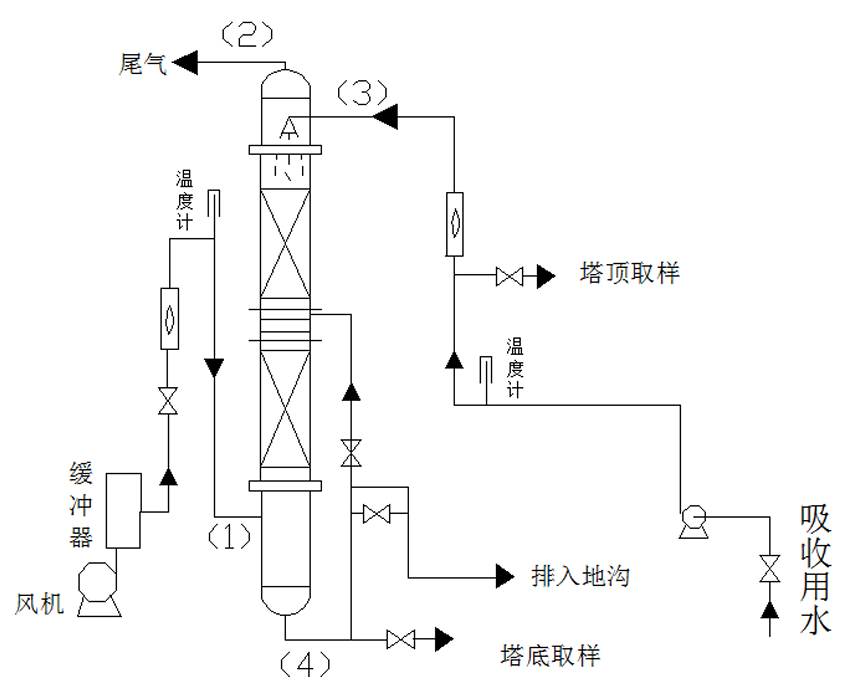
\includegraphics[width=0.8\textwidth]{./figure/吸收塔工艺流程示意图.png}
	\caption{吸收塔工艺流程示意图}
\end{figure}